\documentclass{beamer}
%\documentclass[handout]{beamer}
\usepackage[T1]{fontenc}
\usepackage[english]{babel}
\usepackage[fixlanguage]{babelbib}
\usepackage[utf8]{inputenc}
\usepackage{graphicx}
\usepackage{tikz}
\usepackage[matrix,arrow]{xy}
\usepackage{amsmath}
\usepackage{amssymb}
\usepackage{dsfont}
\usepackage{hyperref}

%\usepackage[T1]{fontenc}
%\usepackage[english]{babel}
%\usepackage[fixlanguage]{babelbib}
%\usepackage{multimedia}



\usetheme{Warsaw}
%\useinnertheme{rounded}
\useoutertheme{infolines}
%\setbeamercovered{transparent}

\title[DEC-PD]{Orientation Fields on Closed Surfaces\\
                A Discrete Exterior Calculus Primal Dual (DEC-PD) Aproach}
\author{Ingo Nitschke}
\institute{IWR - TU Dresden}
%\date{25. September 2014}
\date{\today}

\beamertemplatenavigationsymbolsempty

\newcommand{\R}{\mathds{R}}
\newcommand{\Z}{\mathds{Z}}
\newcommand{\csd}{\text{csd}}
\renewcommand{\div}{\text{Div}}
\renewcommand{\hom}{\text{Hom}}
\newcommand{\err}{\text{Err}}
\newcommand{\id}{\text{Id}}
\newcommand{\D}{\text{D}}
\renewcommand{\d}{\mathrm{d}}
\newcommand{\exd}{\mathbf{d}}
\newcommand{\argmin}{\operatornamewithlimits{argmin}}
\newcommand{\sgn}{\mathop{\mathrm{sgn}}\nolimits}
\newcommand{\formpunkt}{\,\text{.}}
\newcommand{\formkomma}{\,\text{,}}
\newcommand{\formtext}[1]{\quad\text{#1}\quad}
\newcommand{\eps}{\varepsilon}
\newcommand{\vecflat}[1]{\vec{#1}^{\,\flat}}
\newcommand{\vecover}[2]{\vec{#1}^{\,#2}}
\newcommand{\diag}[1]{\text{diag}\left( #1 \right)}
\newcommand{\II}{I \! I}
\newcommand{\av}{\text{Av}}
\newcommand{\conn}{\text{Conn}}
\newcommand{\tred}[1]{\textcolor{red}{#1}}

% IDENTIFIERS for math mode:

%surface (manifold) -> M, S, \Omega 
\newcommand{\M}{M}
%volume element (volume measure) -> \mu, dA, d\Omega
\newcommand{\dA}{dA}
%director field (contra-vector)
\newcommand{\p}{\mathbf{p}}
\newcommand{\q}{\mathbf{q}}
%director field (co-vector, flat of contra-vector)
\newcommand{\pfl}{\mathbf{p}^{\flat}}
\newcommand{\qfl}{\mathbf{q}^{\flat}}
%discrete director field (co-vector, flat of contra-vector)
\newcommand{\pflh}{\mathbf{p}^{\flat}_{h}}
\newcommand{\pflhOld}{\widehat{\mathbf{p}}^{\flat}_{h}}
\newcommand{\qflh}{\mathbf{q}^{\flat}_{h}}
%discrete director field (contra-vector)
\newcommand{\ph}{\mathbf{p}_{h}}
%discrete PD director field (co-vector, flat of contra-vector)
\newcommand{\PDpflh}{\underline{\mathbf{p}}^{\flat}_{h}}
\newcommand{\PDqflh}{\underline{\mathbf{q}}^{\flat}_{h}}
%discrete director field (contra-vector)
\newcommand{\PDph}{\underline{\mathbf{p}}_{h}}
\newcommand{\PDqh}{\underline{\mathbf{q}}_{h}}
%discrete PD director field OLD SOLUTION (co-vector, flat of contra-vector)
\newcommand{\PDpflhOld}{\underline{\widehat{\mathbf{p}}}^{\flat}_{h}}
%discrete director field OLD SOLUTION (contra-vector)
\newcommand{\PDphOld}{\underline{\widehat{\mathbf{p}}}_{h}}
%Frank Oseen Energy (without Lagrange term for normalizing)
\newcommand{\EOS}{E_{\text{FO}}}
%Normalizing energy
\newcommand{\EN}{E_{n}}
%Laplace-Beltrami or Rot-Rot-Laplace
\newcommand{\LB}{\boldsymbol{\Delta}^{\text{\tiny RR}}}
%Laplace-CoBeltrami or Grad-Div-Laplace
\newcommand{\LCB}{\boldsymbol{\Delta}^{\text{\tiny GD}}}
%Laplace-deRham
\newcommand{\LDR}{\boldsymbol{\Delta}^{\text{\tiny dR}}}
%discrete Laplace-Beltrami or Rot-Rot-Laplace
\newcommand{\LBh}{\LB_{h}}
%Laplace-CoBeltrami or Grad-Div-Laplace
\newcommand{\LCBh}{\LCB_{h}}
%Laplace-deRham
\newcommand{\LDRh}{\LDR_{h}}
%Landau symbol
\renewcommand{\O}{\mathcal{O}}
%Vertices
\newcommand{\V}{\mathcal{V}}
%Edges
\newcommand{\E}{\mathcal{E}}
%Faces
\newcommand{\F}{\mathcal{F}}
%Simplicial complex
\newcommand{\K}{\mathcal{K}}
%edge vector
\newcommand{\e}{\mathbf{e}}
%vertex vector
\renewcommand{\v}{\mathbf{v}}
%PD-Basis
\newcommand{\PDxi}{\boldsymbol{\xi}}



\begin{document}
 \frame{ \titlepage }
 \frame {
    \frametitle{Content}
    \tableofcontents
  }

\section{Surface Discretization (Simplicial Complex)} 

  \begin{frame}
    \begin{block}{The surface mesh is made of simplices \( \sigma=v,e,f \):}
      \begin{itemize}
        \item<1-> \alt<1>{\tred{vertices}}{vertices}\alt<2>{, \tred{edges}}{, edges}\alt<3>{, \tred{(triangle) faces}}{, (triangle) faces}
        \item<4->  equipped with an orientation
        \item<5->  have circumcenters \( c(\sigma) \in Int(\sigma) \Rightarrow :  \) well-centered)
        \item<6->  are refinable (circumcentric subdivision) 
      \end{itemize}
    \end{block}
    \begin{overprint}
      \onslide<1> \centering\input{bilder/tikz/S0.tex}
      \onslide<2> \centering\input{bilder/tikz/S1.tex}
      \onslide<3> \centering\input{bilder/tikz/S2.tex}
      \onslide<4> \centering\input{bilder/tikz/SOrient.tex}
      \onslide<5> \centering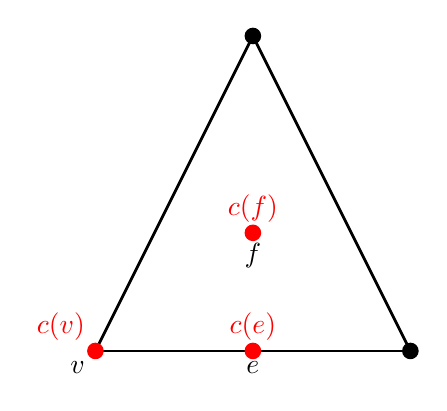
\begin{tikzpicture}[>=latex, scale=2, line width=1pt]
          % Coords
          \coordinate (V0) at (0,0);
          \coordinate (V1) at (2,0);
          \coordinate (V2) at (1,2);
          \coordinate (C01) at (1,0);
          \coordinate (C02) at (0.5,1);
          \coordinate (C12) at (1.5,1);
          \coordinate (C) at (1,0.75);
          % Arrows
          \draw[opacity=1]
            (V0) -- (V1);
          \draw[opacity=1]
            (V1) -- (V2);
          \draw[opacity=1]
            (V2) -- (V0);

		%\fill[red] (V0) -- (V1) -- (V2) -- (V0);
         
          % Points
          \fill[opacity=1](V0) node[below left] {\( v \)};
		  \fill[opacity=1, red](V0) node[above left] {\( c(v) \)} circle (1.5pt);
		  \fill[opacity=0] (V0)  circle (1.5pt);
          \fill[opacity=1] (V1)  circle (1.5pt);
          \fill[opacity=1](V2)   circle (1.5pt);
          \fill[opacity=0] (C02)  circle (1.5pt);
          \fill[opacity=1] (C01) node[below] {\( e \)};
		  \fill[opacity=1, red] (C01) node[above] {\( c(e) \)} circle (1.5pt);
          \fill[opacity=0](C12)  circle (1.5pt);
          \fill[opacity=1](C) node[below] {\( f\)};
		  \fill[opacity=1, red](C) node[above] {\( c(f)\)} circle (1.5pt);	

		 \coordinate (CC2) at (1,0.58);
          \draw[opacity=0, color=red, ->] (CC2) + (135:0.2) arc (135:405:0.2) --++ (-3pt,3pt);
		
		\draw[opacity=0, color=red, ->] (V0) -- (V1);

		\coordinate (CC0) at (1,1.25);
          \draw[opacity=0, color=red, ->] (V0) + (135:0.1) arc (135:405:0.1) --++ (-2pt,2pt);
\end{tikzpicture}

      \onslide<6> \centering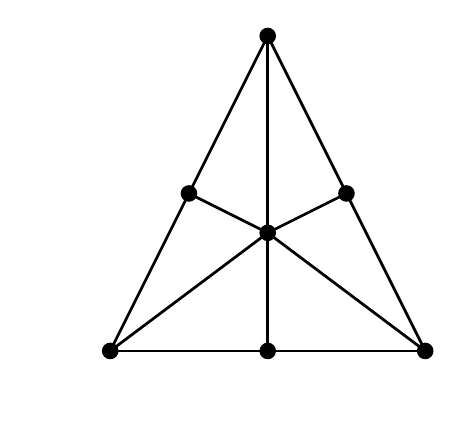
\begin{tikzpicture}[>=latex, scale=2, line width=1pt]
          % Coords
          \coordinate (V0) at (0,0);
          \coordinate (V1) at (2,0);
          \coordinate (V2) at (1,2);
          \coordinate (C01) at (1,0);
          \coordinate (C02) at (0.5,1);
          \coordinate (C12) at (1.5,1);
          \coordinate (C) at (1,0.75);
          % Arrows
          \draw[line width=1pt]
            (V0) -- (V1);
          \draw[line width=1pt]
            (V1) -- (V2);
          \draw[line width=1pt]
            (V2) -- (V0);
          \draw[line width=1pt]
            (V0) -- (C);
          \draw[line width=1pt]
            (V1) -- (C);
          \draw[line width=1pt]
            (V2) -- (C);
          \draw[line width=1pt]
            (C01) -- (C);
          \draw[line width=1pt]
            (C02) -- (C);
          \draw[line width=1pt]
            (C12) -- (C);
          % Points
          \fill (V0) circle (1.5pt);
          \fill (V1) circle (1.5pt);
          \fill (V2) circle (1.5pt);
          \fill (C01) circle (1.5pt);
          \fill (C02) circle (1.5pt);
          \fill (C12) circle (1.5pt);
          \fill (C) circle (1.5pt);


			%wegen abmessung
			          % Coords
          \coordinate (V0) at (0,0);
          \coordinate (V1) at (2,0);
          \coordinate (V2) at (1,2);
          \coordinate (C01) at (1,0);
          \coordinate (C02) at (0.5,1);
          \coordinate (C12) at (1.5,1);
          \coordinate (C) at (1,0.75);
          % Arrows
          \draw[opacity=0]
            (V0) -- (V1);
          \draw[opacity=0]
            (V1) -- (V2);
          \draw[opacity=0]
            (V2) -- (V0);
         
          % Points
          \fill[opacity=0](V0) node[below left] {\( \sigma^0 \)};
		  \fill[opacity=0](V0) node[above left] {\( c(\sigma^0) \)} circle (1.5pt);
          \fill[opacity=0, color=red] (V0)  circle (1.5pt);
          \fill[opacity=0] (V1)  circle (1.5pt);
          \fill[opacity=0](V2)   circle (1.5pt);
          \fill[opacity=0] (C02)  circle (1.5pt);
          \fill[opacity=0] (C01) node[below] {\( \sigma^1 \)};
		  \fill[opacity=0] (C01) node[above] {\( c(\sigma^1) \)} circle (1.5pt);
          \fill[opacity=0](C12)  circle (1.5pt);
          \fill[opacity=0](C) node[below] {\( \sigma^2\)};
		  \fill[opacity=0](C) node[above] {\( c(\sigma^2)\)} circle (1.5pt);	

		 \coordinate (CC2) at (1,1.25);
          \draw[opacity=0, ->] (CC2) + (135:0.15) arc (135:405:0.15) --++ (-3pt,3pt);
		
		\draw[opacity=0, ->] (V0) -- (V1);

		\coordinate (CC0) at (1,1.25);
          \draw[opacity=0, ->] (V0) + (135:0.1) arc (135:405:0.1) --++ (-2pt,2pt);

\end{tikzpicture}
    \end{overprint}
  \end{frame}

  \begin{frame}
    \begin{block}{The surface mesh is a well-centered oriented manifold-like simplicial complex \( \K \):}
      \begin{itemize}
        \item<1-> \textbf{simplicial complex} \( \K=\V\cup\E\cup\F \): "like a triangulation"    
        \item<2-> \textbf{well-centered}: faces are well-centered (maximum angle less than \( 90^{\circ} \))
        \item<3-> \textbf{oriented}: neighboured faces have the same orientation
        \item<4-> \textbf{manifold-like}: polyhedron \( \bigcup_{f\in\F}f \) is a \( C^{0} \)-manifold
      \end{itemize}
    \end{block}
    \begin{overprint}
      \onslide<1> \centering\input{bilder/tikz/ExampleSC.tex}
      \onslide<2> \centering\input{bilder/tikz/ExampleSCCircums.tex}
      \onslide<3> \centering\input{bilder/tikz/ExampleSCOrient.tex}
      \onslide<4> 
          \centering\includegraphics[width=0.3\textwidth]{bilder/Icosahedron.pdf}\footnotetext{https://commons.wikimedia.org/wiki/File:Icosahedron.svg}
    \end{overprint}
  \end{frame}


\section{Introduction in required DEC topics}

  \subsection{Shopping List}
    
    \begin{frame}
      \begin{block}{PDE for orientation fields}
        \begin{overprint}
          \onslide<1>
            \begin{align*}
              \partial_{t}\pfl = \left( K_{1}\LCB + K_{3}\LB\right)\pfl - K_{n} \left( \left\| \pfl \right\|^{2} - 1 \right)\pfl
            \end{align*}
          \onslide<2>
            \begin{align*}
              \partial_{t}\tred{\pfl} = \left( K_{1}\LCB + K_{3}\LB\right)\tred{\pfl} 
                        - K_{n} \left( \left\| \tred{\pfl} \right\|^{2} - 1 \right)\tred{\pfl}
            \end{align*}
          \onslide<3>
            \begin{align*}
              \partial_{t}\pfl = \left( K_{1}\tred{\LCB} + K_{3}\tred{\LB}\right)\pfl - K_{n} \left( \left\| \pfl \right\|^{2} - 1 \right)\pfl
            \end{align*}
        \end{overprint}
        We need to discretize
        \begin{itemize}
          \item<2-> the \alt<2>{\tred{1-form \( \pfl \)}}{1-form \( \pfl \)}\( \in\Lambda^{1}(\M) \)
          \item<3-> the \alt<3>{Laplace-Operators \tred{\( \LCB \)} and \tred{\( \LB \)}}{Laplace-Operators \( \LCB \) and \( \LB \)}
        \end{itemize}
      \end{block}
      \footnotetext{\( \LCB \)...Vector-Laplace-CoBeltrami-Operator or Grad-Div-Laplace}
      \footnotetext{\( \LB \)...Vector-Laplace-Beltrami-Operator or Rot-Rot-Laplace}
    \end{frame}
  

\end{document}
